% Copyright 2004 by Till Tantau <tantau@users.sourceforge.net>.
%
% In principle, this file can be redistributed and/or modified under
% the terms of the GNU Public License, version 2.
%
% However, this file is supposed to be a template to be modified
% for your own needs. For this reason, if you use this file as a
% template and not specifically distribute it as part of a another
% package/program, I grant the extra permission to freely copy and
% modify this file as you see fit and even to delete this copyright
% notice. 

%\documentclass[11pt]{beamer}
\documentclass{beamer}

%\usepackage[absolute,overlay]{textpos}
\usepackage{array} % needed for \arraybackslash
\usepackage{graphicx}
\usepackage{pdfpages}

%\usepackage{adjustbox} % for \adjincludegraphics

% There are many different themes available for Beamer. A comprehensive
% list with examples is given here:
% http://deic.uab.es/~iblanes/beamer_gallery/index_by_theme.html
% You can uncomment the themes below if you would like to use a different
% one:
%\usetheme{Madrid}
%\usecolortheme{orchid}
\usenavigationsymbolstemplate{}

%\setbeamertemplate{footline}[page number] 
%\setbeamertemplate{navigation symbols}{} 


\title{NDN Hackathon}

% A subtitle is optional and this may be deleted
\subtitle{NDN-RTC Congestion Control Design}

\author{Hila B. Abraham, Peter Gusev, Chengyu Fan, Guilio Grassi, Klaus Schneider}
% - Give the names in the same order as the appear in the paper.
% - Use the \inst{?} command only if the authors have different
%   affiliation.

\institute[Universities of Somewhere and Elsewhere] % (optional, but mostly needed)
{
  NDN Retreat 2016\\
  UCSD, San Diego 
  }
% - Use the \inst command only if there are several affiliations.
% - Keep it simple, no one is interested in your street address.

\date{\today}
% - Either use conference name or its abbreviation.
% - Not really informative to the audience, more for people (including
%   yourself) who are reading the slides online

%\subject{Theoretical Computer Science}
% This is only inserted into the PDF information catalog. Can be left
% out. 

% If you have a file called "university-logo-filename.xxx", where xxx
% is a graphic format that can be processed by latex or pdflatex,
% resp., then you can add a logo as follows:

% \pgfdeclareimage[height=0.5cm]{university-logo}{university-logo-filename}
% \logo{\pgfuseimage{university-logo}}

% Delete this, if you do not want the table of contents to pop up at
% the beginning of each subsection:
\AtBeginSubsection[]
{
  \begin{frame}<beamer>{Outline}
    \tableofcontents[currentsection,currentsubsection]
  \end{frame}
}

% Let's get started
\begin{document}

\begin{frame}
  \titlepage
\end{frame}

\section{Introduction}

\begin{frame}{Outline}
	
	
	
	\large
\textbf{Motivation: Figure out what is wrong with NDN-RTC
}
~\\
	\begin{enumerate}
		\item RTT Estimation
		\item Fixed rate thresholds ($\lambda_{min}, \lambda_{max}$)
		\item Effect of NFD Access Strategy
	\end{enumerate}
	~\\
	
	Future work: Don't put Generation Delay into Cache
	
\end{frame}


\begin{frame}{RTT Averaging is too slow}
	
	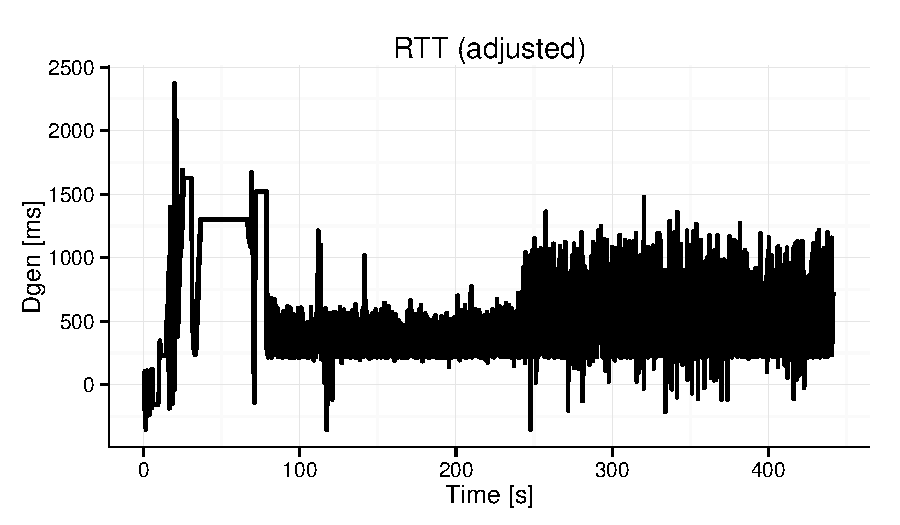
\includegraphics[width=\linewidth,page=1]{images/test8_1.pdf}
	
\end{frame}

\begin{frame}{RTT Averaging is too slow}
	
	\includegraphics[width=\linewidth,page=2]{images/test8_1.pdf}
	
\end{frame}

\begin{frame}{Result: Playout buffer doesn't adjust correctly}
	
	\includegraphics[width=\linewidth,page=6]{images/test8_1.pdf}
	
\end{frame}


\begin{frame}{Problem: Fixed Rate Thresholds (``Lambda'')}
	
	\includegraphics[width=\linewidth,page=7]{images/test8_1.pdf}
	
	\textbf{Trade-Off: Reaching fresh data $\Leftrightarrow$ Causing Congestion}
	\begin{itemize}
	\item[$\Rightarrow$] More adaptive congestion window + consider buffer size
%	\item[$\Rightarrow$] Rate-based design
	\end{itemize} 
\end{frame}


\begin{frame}{Access Strategy causes huge problems}
	
	\includegraphics[width=\linewidth,page=2]{images/test8_5.pdf}
	\textbf{
	Access Strategy suppresses Retx for 100 ms!}
	
\end{frame}


\begin{frame}{Access Strategy causes huge problems}
	
	\includegraphics[width=\linewidth,page=8]{images/test8_5.pdf}
	
\end{frame}


\begin{frame}{Access Strategy causes huge problems}
	
	\includegraphics[width=\linewidth,page=6]{images/test8_5.pdf}
	
\end{frame}


\begin{frame}{Future Work: Data Gen Delay}
	
	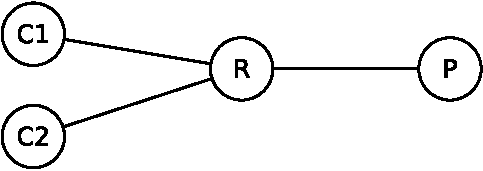
\includegraphics[width=\linewidth,page=1]{images/fib_agg.pdf}
	~\\[1em]
	
	\large
	\textbf{Data Generation Delay is used for RTT Estimation!
	}
	~\\[1em]
	
	\Large
	
	$RTT_{est} = RTT_{raw} - D_{gen}$
\end{frame}


\begin{frame}{Result: Adjusted RTT becomes Negative!}
	
	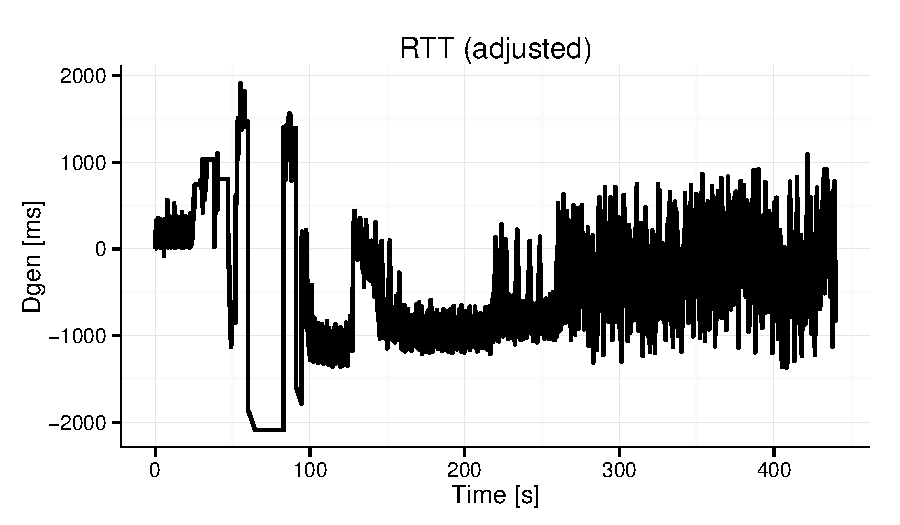
\includegraphics[width=\linewidth,page=1]{images/test8_5.pdf}
	
\end{frame}

\begin{frame}{Workaround: NDNLP Tags}
	
	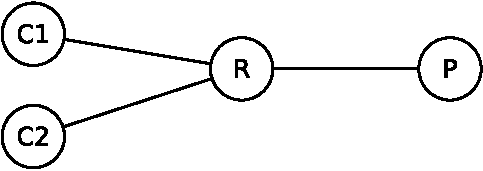
\includegraphics[width=\linewidth,page=1]{images/fib_agg.pdf}
	
	\begin{itemize}
		\item Can't manipulate data packet
		\item[$\Rightarrow$] Add NDNLP Header
	\end{itemize}
	
\end{frame}

\begin{frame}{Done}
	\LARGE
	
	Thanks a lot!
	
\end{frame}



\end{document}

